\documentclass{article}
\usepackage[utf8]{inputenc}
\usepackage{physics}
\usepackage{amsmath}
\usepackage{showlabels}
\title{Statistical Computing for Scientists and Engineers\\[1em] Homework 1}
\author{Jiale Shi}
\date{September/11/2018}

\usepackage{natbib}
\usepackage{graphicx}

\begin{document}

\maketitle

\newpage
\section{Problem 1}
Consider $n$ samples $D_{n} = (x_{1},...,x_{n})$, independently drawn from normal distribution, $N_{\mu, \sigma^{2}})$, with known variance and unknown mean, $\sigma^{2}$ and $\mu$, respectively. Assume that the mean has a prior given by the normal distribution:

\begin{equation}
p(\mu|m,v^{2})= N(\mu|m,v^{2}) \propto \exp(\frac{1}{2v^{2}} (\mu-m)^2)
%\pdv[2]{u}{x}+\pdv[2]{u}{y} = 0
\end{equation}

Derive the posterior:

\begin{equation}
p(\mu|D) \sim N(\mu_{n},\sigma^{2}) 
\end{equation}

\begin{equation}
\mu_{n} = \sigma^{2}\left(\frac{m}{v^{2}}+\frac{n\Bar{x}}{\sigma^{2}}\right), \sigma_{n}^{2} = \frac{1}{\frac{n\Bar{x}}{\sigma^{2}}+\frac{1}{v^2}}
\end{equation}

in which $\Bar{x}$ is the empirical mean $(\Bar{x}=\sum^n_{i=1}x_{i})$.

Answer:
\begin{equation}
\begin{aligned}
    p(\mu|D) &= \prod_{i=1}^{n} f(x_{i}|\mu) p(\mu) \\
    &\propto \exp{-\frac{\sum_{i=1}^{n}(x_{i}-\mu)^2}{2\sigma^{2}} - \frac{(\mu-m)}{2v^2}} \\
     &\propto \exp{-\frac{\mu^2}{2}(\frac{n}{\sigma^2}+\frac{1}{v^2})+\mu(\frac{\sum_{i}^{n}x_i}{\sigma^2}+\frac{m}{v^2})} \\
    &\propto \exp{-\frac{\mu^2}{2}(\frac{n}{\sigma^2}+\frac{1}{v^2})+\mu(\frac{n\Bar{x}}{\sigma^2}+\frac{m}{v^2})} \\
    &\propto \exp{-\frac{1}{2\sigma_{n}^{2}}(\mu-\mu_{n})}
\end{aligned}
\end{equation}
\begin{equation}
\frac{1}{\sigma_{n}^{2}} = \frac{1}{v^2}+\frac{n}{\sigma^2} \Rightarrow{} \sigma_{n}^{2} = \frac{1}{\frac{1}{v^2}+\frac{n}{\sigma^2}}
\end{equation}
\begin{equation}
    \mu_n = \sigma_{n}^2\left(\frac{m}{v^2}+\frac{n\Bar{x}}{\sigma^2}\right) = \left(\frac{1}{\frac{1}{v^2}+\frac{n}{\sigma^2}}\right)\left(\frac{m}{v^2}+\frac{n\Bar{x}}{\sigma^2}\right)
\end{equation}



\newpage
\section{Problem 2}
Consider a univariate Gaussian $N(X|\mu, \lambda^{-1})$ and a dataset $X = \{x_{1}, x_{2}, x_{3},...,x_{N}\}$, $x_{i}\sim N(X|\mu,\lambda^{-1})$ of i.i.d observations. Write down the likelihood for this model and show that a conjugate prior is of the form:

\begin{equation}
    p(\mu,\lambda)\propto \left[\lambda^{1/2} \exp(-\frac{\lambda \mu^{2}}{2})\right]^{\beta} \exp(c\lambda \mu - d\lambda)
\end{equation}

where $c$, $d$, $\beta$ are constants. Given $p(\mu,\lambda) = p(\mu\mid\lambda) p(\lambda)$, we can recognize that the above prior is the product of a Gaussian $p(\mu\mid\lambda)$ whose precision is a linear function of $\lambda$ and of the gamma distribution $p(\lambda)$. As a result the normalized prior take the form:
\begin{equation}
p(\mu, \lambda) = N \left( \mu\mid \mu_{0},(\beta \lambda)^{-1}\right) Gam(\lambda\mid a,b)  
\end{equation}
where $\mu_{0}=c/\beta, \alpha = 1+\beta/2$ and $b = d-c^2/2\beta$. Show that the posterior $p(\mu, \lambda \mid X)$ is also a Gaussian-gamma distribution of the same functional form as thr prior:
\begin{equation}
    N(\mu \mid \mu_N, ((N+\beta)\lambda)^-1) Gam(\lambda \mid a_N, b_N)
\end{equation}
write down expressions for the parameters of this posterior distribution $\mu_N$, $a_N$ and $b_N$

Answer:
the likelihood takes the form:
\begin{equation}
\begin{aligned}
    p(X|\mu, \lambda) & = \prod_{n=1}^{N} f(x_{n}|\mu) \propto \lambda^{N/2}\exp{-\frac{1}{2}\lambda \sum_{n=1}^N(x_{n}-\mu)^2}\\ & \propto \left[\lambda^{1/2} \exp{-\frac{\lambda \mu^2}{2}}\right]^{N} \exp{\lambda\mu\sum_{n=1}^{N}x_{n}-\frac{1}{2}\lambda\sum_{n=1}^{N}x_{n}^{2}}
\end{aligned}
\end{equation}

we need a prior that has a similar functional form in terms of $\lambda$ and $\mu$.

\begin{equation}
\begin{aligned}
&\beta = N \\
&c = \sum_{n=1}^{N}x_{n} \\
&d = \frac{1}{2}\sum_{n=1}^{N}x_{n}^{2}\\
&p(\mu,\lambda)\propto \left[\lambda^{1/2} \exp(\frac{\lambda \mu^{2}}{2})\right]^{\beta} \exp(c\lambda \mu - d\lambda)
\end{aligned}
\end{equation}

\begin{equation}
\begin{aligned}
p(\mu,\lambda) &\propto \left[\lambda^{1/2} \exp(\frac{\lambda \mu^{2}}{2})\right]^{\beta} \exp(c\lambda \mu - d\lambda) \\
& = (\beta\lambda)^{1/2} \exp{-\frac{\beta \lambda}{2}\left(\mu - \frac{c}{\beta}\right)^{2}} \lambda^{(\beta-1)/2} \exp{-\left(d-\frac{c^2}{2\beta}\right)\lambda} \\
& = p(\mu|\lambda) p(\lambda) \\
& = N\left(\mu| \mu_{0}=\frac{c}{d}, \sigma = (\beta \lambda)^{-1}\right) Gamma\left(\lambda|a = \frac{1+\beta}{2},b = d-\frac{c^2}{2\beta}\right)
\end{aligned}
\end{equation}

\begin{equation}
\begin{aligned}
p(\mu,\lambda|X) &\propto \lambda^{N/2}\lambda^{a-1}\exp\left[-\left(b+\frac{1}{2}\sum_{n=1}^{N}x_{n}^{2}+\frac{\beta}{2}\mu_{0}^{2}\right)\lambda\right]\times \\
&[\lambda(N+\beta)]^{1/2}\exp{-\frac{\lambda(N+\beta)}{2}\left[\mu^{2}-\frac{2}{N+\beta}(\beta\mu_{0}+\sum_{n=1}^{N}x_{n})\mu\right]} \\
& = N(\mu | \mu_{N},[\lambda(N+\beta)]^{-1}) Gam(\lambda | a_{N},b_{N}) \\
\end{aligned}
\end{equation}

\begin{equation}
\begin{aligned}
& \mu_{N}= -\frac{\beta\mu_{0}+\sum_{n=1}^{N}x_{n}}{N+\beta}\\
& a_{N} = \frac{N}{2}+a\\
& b_{N} = -\left(b+\frac{1}{2}\sum_{n=1}^{N}x_{n}^{2}+\frac{\beta}{2}\mu_{0}^{2}-\frac{(\beta\mu_{0}+\sum_{n=1}^{N}x_{n})^{2}}{2(N+\beta)}\right)
\end{aligned}
\end{equation}


\newpage
\section{Problem 3}
The Wishart distribution distribution $W_m(n,\Sigma)$.

1. To prove $E[X|n,\Sigma]=n\Sigma$.


$X = \sum_{i=1}^{n} z_{i}z_{i}^{T} \sim W_{m}(n,\Sigma)$, where $z_{1},...,z_{n} \sim N_{m}(0,\Sigma)$, and $z_{1},...,z_{n}$ are independent with each other.
\begin{equation}
    E[X|n,\sum] =E[\sum_{1}^{n}z_{i}z_{i}^{T}] = \sum_{1}^{n}E[z_{1}z_{1}^{T}] = \sum_{1}^{n} Var(z_{1}) = n\Sigma
\end{equation}

Therefore,$E[X|n,\Sigma]=n\Sigma$.

2. To prove $Cov[X] = 2n\Sigma \bigotimes \Sigma$.

\begin{equation}
\begin{aligned}
    Cov(X) &= Cov\left(\sum_{i=1}^{n} z_{i}z_{i}^{T}\right) \\
    &= \sum_{1}^{n}Cov\left(z_{1}z_{1}^{T}\right) \\
    &= n Cov\left(z_{1}z_{1}^{T}\right)  \\
    &= n Cov\left(z_{1} \boxed{ } z_{1}\right) \\
    &= n Cov((\Sigma \bigotimes \Sigma)(x \boxed{ } x)) \\
    &= 2n\Sigma \bigotimes \Sigma
\end{aligned}
\end{equation}

\newpage
\section{Problem 4}
(a) Derive the log Gamma distribution $Y \sim log[X]$, $X= G(\alpha, \beta)$ and show that it belongs to both families above.

Answer:
$Y \sim log[X]$, $X= G(\alpha, \beta)$, therefore, $X \sim \exp[Y]$.
\begin{equation}
\begin{aligned}
    f_{Y}(x) & = f_{X=e^Y} (e^x) \frac{d e^x}{d x} = \frac{1}{\Gamma(\alpha)} e^{-\beta e^x}(\beta e^{x})^{\alpha} \\
    & = \frac{\beta^{\alpha}}{\Gamma(\alpha)} e^{-\beta e^x}(e^{x})^{\alpha}
\end{aligned}
\end{equation}

Check whether it belongs to exponential family.
\begin{equation}
\begin{aligned}
    \frac{\beta^{\alpha}}{\Gamma(\alpha)} e^{-\beta e^x}(e^{x})^{\alpha} & = \frac{\beta^{\alpha}}{\Gamma(\alpha)} \exp{-\beta e^x+x\alpha} \\
    & = \frac{\beta^{\alpha}}{\Gamma(\alpha)} \exp{(-\beta,\alpha)(e^x,x)^{T}} \\
    & = \frac{\beta^{\alpha}}{\Gamma(\alpha)} \exp{\eta(\alpha,\beta)^{T}u(x)} 
\end{aligned}
\end{equation}
where $u(x)=(e^x,x)^T, \eta(\alpha,\beta)=(-\beta,\alpha)^{T}, h(x)=1,g(\alpha,\beta)=\frac{\beta^{\alpha}}{\Gamma(\alpha)} $. Therefore, the log Gamma distribution $Y$ belongs to the exponential family.
\newline
(b) Provide examples of two distributions that part of the exponential family.

Answer:
Consider the Bernoulli Distribution
\begin{equation}
\begin{aligned}
  p(x|\mu) & =  \mu^{x}(1-\mu)^(1-x) \\
  & = \exp{x\ln{\mu}+(1-x)\ln\left(1-\mu\right)} \\
  & = (1-\mu)\exp{\ln\left(\frac{\mu}{1-\mu}\right)x}
\end{aligned}
\end{equation}

\begin{equation}
\begin{aligned}
&\eta = \ln\left(\frac{\mu}{1-\mu}\right) \\
&\mu = \sigma(\eta)= \frac{1}{1+e^{-\eta}} \\
& g(\eta) = 1-\mu = \frac{1}{1+e^{\eta}} \\
& p(x|\mu) = g(\eta)\exp{\eta x}, \mu(x)= x, h(x)=1,g(\eta) = 1-\mu = \frac{1}{1+e^{\eta}}
\end{aligned}
\end{equation}

Consider the Beta distribution

\begin{equation}
\begin{aligned}
  p(x|a,b) & =  \frac{\Gamma(a+b)}{\Gamma(a)\Gamma(b)} x^{a-1}(1-x)^{b-1} \\
  & = \frac{\Gamma(a+b)}{\Gamma(a)\Gamma(b)} \exp[(a-1)\ln(x) + (b-1)\ln(1-x)] \\
  & = h(x)g(\eta)\exp{\eta^{T}u(x)}
\end{aligned}
\end{equation}

\begin{equation}
\begin{aligned}
&\eta = (a-1,b-1)^{T} \\
&\mu(x) = (\ln(x),\ln(1-x))^{T} \\
& g(a,b) = \frac{\Gamma(a+b)}{\Gamma(a)\Gamma(b)} \\
& h(x)=1
\end{aligned}
\end{equation}
\newline
(c) Provide examples of two distributions that are part of the local-scale family.

Answer:

Consider the Cauchy distribution:
take $\Psi(x) = \frac{1}{\pi}\frac{1}{1+x^2}$
\begin{equation}
\begin{aligned}
p(x|a,b) = \frac{1}{b}\Psi\left(\frac{x+a}{b}\right) = \frac{1}{\pi b}\frac{1}{1+\left(\frac{x+a}{b}\right)^2}
\end{aligned}
\end{equation}
defines the Cauchy L-S family.

Consider the Uniform distribution:
take $\Psi(x) = I_{(0,1)}(x)$
\begin{equation}
\begin{aligned}
    I_{(0,1)}(x) = 1, if 0<x<1
    I_{(0,1)}(x) = 0, otherwise
\end{aligned}
\end{equation}
$\Psi(x)$ is the pdf of the Unif(0,1) distribution
\begin{equation}
\begin{aligned}
p(x|a,b) = \frac{1}{b}\Psi\left(\frac{x+a}{b}\right) = \frac{1}{b}I_{(0,1)}\left(\frac{x+a}{b}\right) = \frac{1}{b}I_{(-a,-a+b)}(x)
\end{aligned}
\end{equation}
This is the pdf of the Unif$(-a,-a+b)$
\newpage
\section{Problem 5}
(a) Start by plotting a histogram of the camera's max resolution. Fit a normal distribution to this data and plot the fitted distribution on top of histogram. Repeat for the camera weight.

Answer:
the camera's max resolution
\begin{figure}[ht]
\centering
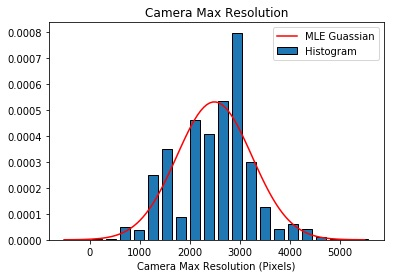
\includegraphics[scale=0.5]{w5a1.jpg}
\caption{Histogram and normal distribution fitting of the camera's max resolution}
%\label{fig:universe}
\end{figure}

the camera's weight
\begin{figure}[ht]
\centering
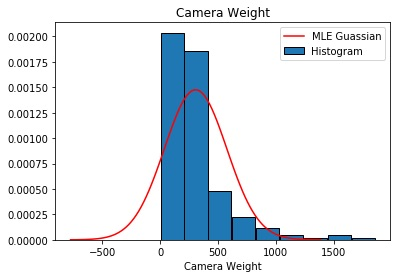
\includegraphics[scale=0.5]{w5a2.jpg}
\caption{Histogram and normal distribution fitting of the camera's weight}
%\label{fig:universe}
\end{figure}
\newline
(b) Standardize the camera max resolution data using the fitted mean, $\Bar{x_{i}}$, and standard deviation, $\sigma_{i}$. This can be completed by computing $(x_{ij}-\Bar{x_{i}})/\sigma_{i}$. Plot a standard Gaussian $N(0,1)$ on top of the normalized data. Comment on why we would be interested in doing this.

Answer:
from (a) the normal distribution fitting for the max resolution
$\Bar{x_i} = 2491.7618497109806, \sigma_{i} = 752.5256308818603$.
Then, we standardize the camera max resolution data by computing $(x_{i}-\Bar{x_{i}})/\sigma_{i}$.

\begin{figure}[ht]
\centering
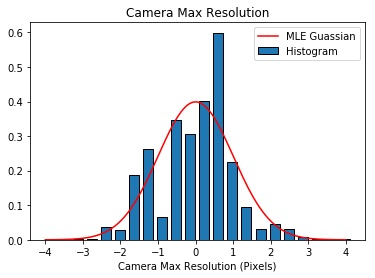
\includegraphics[scale=0.5]{w5b1.jpg}
\caption{Standard Gaussian $N(0,1)$ fitting of the normalized camera's max resolution}
%\label{fig:universe}
\end{figure}


The reason that we would be interested in doing this is that the standardized data is easier to compare with each other.
\newline
(c) Fit a Gamma, $G(\alpha, \beta)$, distribution to the histogram of the camera's weight through MLE. Plot both fitted distributions on top of the histogram. Comment on which distribution provides a better fit.

start by finding the log-likelihood of Gamma distribution
\begin{equation}
  f=\ln(T) = (\alpha-1) \sum \ln(x)  - n\ln(\Gamma(\alpha)) - n\alpha \ln(\beta)-\frac{1}{\beta}\sum x 
\end{equation}
\begin{equation}
  \frac{d\ln(T)}{d\beta} =  -\frac{n\alpha}{\beta}+\frac{1}{\beta^2}\sum x =0 
\end{equation}
\begin{equation}
  \beta = \frac{\sum x}{n \alpha} = \frac{\Bar{x}}{\alpha}
\end{equation}
\begin{equation}
\begin{aligned}
  f(\alpha) &= (\alpha-1)n \Bar{\ln(x)} - n \ln(\Gamma(\alpha))-n\alpha \ln(\frac{\Bar{x}}{\alpha})-n\alpha 
\end{aligned}
\end{equation}
Using the minka-newton method from the paper provided.
\begin{equation}
\begin{aligned}
  f^{'}(\alpha) &= n \Bar{\ln(x)} - n \Psi(\alpha)-n \ln(\Bar{x})+n\ln(\alpha)
\end{aligned}
\end{equation}
\begin{equation}
\begin{aligned}
  f^{''} (\alpha)&=  - n \Psi^{'}(\alpha)+\frac{n}{\alpha}
\end{aligned}
\end{equation}
\begin{equation}
\begin{aligned}
  \frac{1}{\alpha^{new}} = \frac{1}{\alpha^{old}}+ \frac{f^{'}(\alpha)}{\alpha^2 f^{''}(\alpha)} = \frac{1}{\alpha^{old}}+ \frac{ \Bar{\ln(x)} -  \Psi(\alpha)- \ln(\Bar{x})+\ln(\alpha)}{-  \alpha^{2}\Psi^{'}(\alpha)+\alpha}
\end{aligned}
\end{equation}

\begin{figure}[ht]
\centering
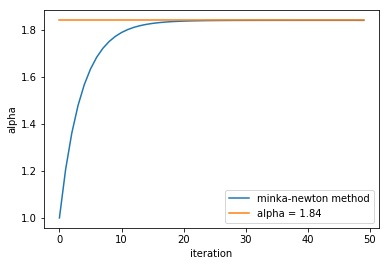
\includegraphics[scale=0.5]{alpha.jpg}
\caption{ alpha value with minka-newton method}
%\label{fig:universe}
\end{figure}
From Figure 4, we find that the value of $\alpha$ converges very quickly. $\alpha \approx 1.84$ and $\beta \approx 166.6387422858897$.

Then we use the $\alpha$ and $\beta$ to plot the fitted Gamma distribution and compare with the Gaussian in Figure 2.
\begin{figure}[ht]
\centering
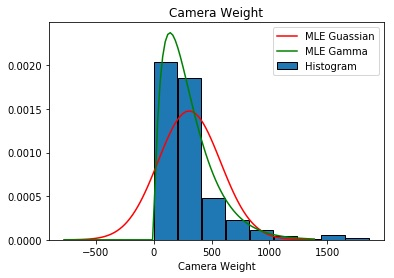
\includegraphics[scale=0.5]{h5c.jpg}
\caption{ Gamma distribution and Gaussian distribution camera's weight}
%\label{fig:universe}
\end{figure}
After comparing with the Gaussian distribution fitting, we find that the Gamma distribution is better than the Gaussian distribution for the camera's weight.
\newline
(d)Plot the camera's release year vs. max-resolution. Fit a 2D Gaussian distribution to this data through MLE. Plot the fitted Gaussian on top of the data.
\begin{figure}[ht]
\centering
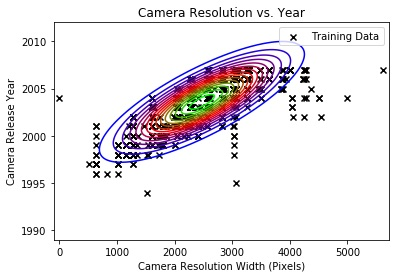
\includegraphics[scale=0.5]{w5d.jpg}
\caption{ 2D Gaussian distribution camera's release year vs. max-resolution}
%\label{fig:universe}
\end{figure}
\newline

%\bibliographystyle{plain}
%\bibliography{references}
\end{document}
